\chapter{Folgen und Konvergenz} $(a_1, a_2 \ldots a_n)$ $a_n$ Zahlen

\section{Definition 1} 


Eine (reelle) Folge ist eine Funktion $f: \N \rightarrow \R, n \mapsto f(n) =: a_n$

\subsubsection{Notation:} $a_n = f(n)$, $(a_n)_{n \in \N}$, $(a_n)_n$
\subsubsection{Bemerkung:} $(a_n)_n$ ist nicht $\{a_1, a_2, \ldots\}$ z.B. $a_n = 1 \implies \{a_1, a_2, \ldots\} = \{1\}$

\section{Definition 2: Konvergenz:}

Sei $(a_n)_n$ eine Folge reellen Zahlen $(a_n)_n$ konvergiert gegen $L \in \R$

Genau dann, wenn: $\forall \epsilon > 0 \exists k_\epsilon \in \N: \forall n \geq k_\epsilon: |a_n - L| < \epsilon$

\textbf{Schreiben} 
\[a_n \to L, n\to \infty, \text{ oder } a_n \to L\]
\[\lim_{n \to \infty} a_n = L, \lim a_n = L\]

$(a_n)_n$ ist divergent, wenn sie nicht konvergiert.

\subsubsection{Alternative Definitionen} 

\begin{align*}
                      & \left(\forall \epsilon > 0 \exists k_\epsilon \in \N: \forall n \geq k_\epsilon: |a_n - L| < \epsilon \right) \\
  \Longleftrightarrow & \left(\forall \epsilon > 0 \exists k_\epsilon \in \N: \forall n \geq k_\epsilon: |a_n - L| \leq \epsilon \right) \\
  \Longleftrightarrow & \left(\forall l \in \N \exists k_\epsilon \in \N: \forall n \geq k_\epsilon: |a_n - L| < \frac{1}{l} \right) \\
  \Longleftrightarrow & \left(\forall l \in \N \exists k_\epsilon \in \N: \forall n \geq k_\epsilon: |a_n - L| \leq \frac{1}{l} \right) 
\end{align*}

\begin{example}
  \begin{enumerate}
    \item Konstante Folge $a_n=a$
      
      $\forall n \quad a_n \to a$
      
      Sei $\epsilon \geq 0$
      
      setze $k_\epsilon=1 \implies |a_n-a|=|a-a|=0<\epsilon$
      
      $\forall n \geq 1$
    \item $\lim_{n \to \infty} \frac{1}{x}=0$ Da $\N \subset \R$ unbeschränkt sind (Satz 1,23)
    
    $\implies$ Für $\epsilon > 0 \exists k_\epsilon \in \N,$
    $k_\epsilon > \frac{1}{\epsilon}$
    
    $\implies$ Für $n \geq k_\epsilon: |\frac{1}{n}-0|=\frac{1}{n}\leq \frac{1}{k_\epsilon}<\epsilon$
    
    \item $(a_n)_n, \quad (a_n)=(-1)^n$ divergent.
    
    \textbf{Angenommen:} Es konvergiert, $\implies \exists L \in \R$
    
    $\forall \epsilon > 0: \exists k_\epsilon : |a_n - L| < \epsilon  \quad \forall n \geq k_\epsilon$ 

    2 Fälle: $L \geq 0$ und $L<0$.
    
    \textbf{Fall $L \geq 0$:} nehme $\epsilon = \frac{1}{2}$ und $k_\frac{1}{2} \in \N: \forall n \geq k_\frac{1}{2}:|a_n-L|<\frac{1}{2}$
    
    Ist $n$ ungerade und $\geq k_\frac{1}{2}$
    
    $\implies \frac{1}{2} > |a_n-L|=|-1-L|=1+L \geq 1 > \frac{1}{2} \lightning$
    
    \textbf{Fall $L < 0$:} nehmen $\epsilon = \frac{1}{2}, k_\frac{1}{2}:|a_n-L|<\frac{1}{2} \quad \forall n \geq k_\frac{1}{2}$
    
    Ist $n$ gerade
    
    $\implies \frac{1}{2} > |a_n-L|=|1-L|=1-L>1 \lightning$
    
    \begin{figure}[!ht]
      \centering
        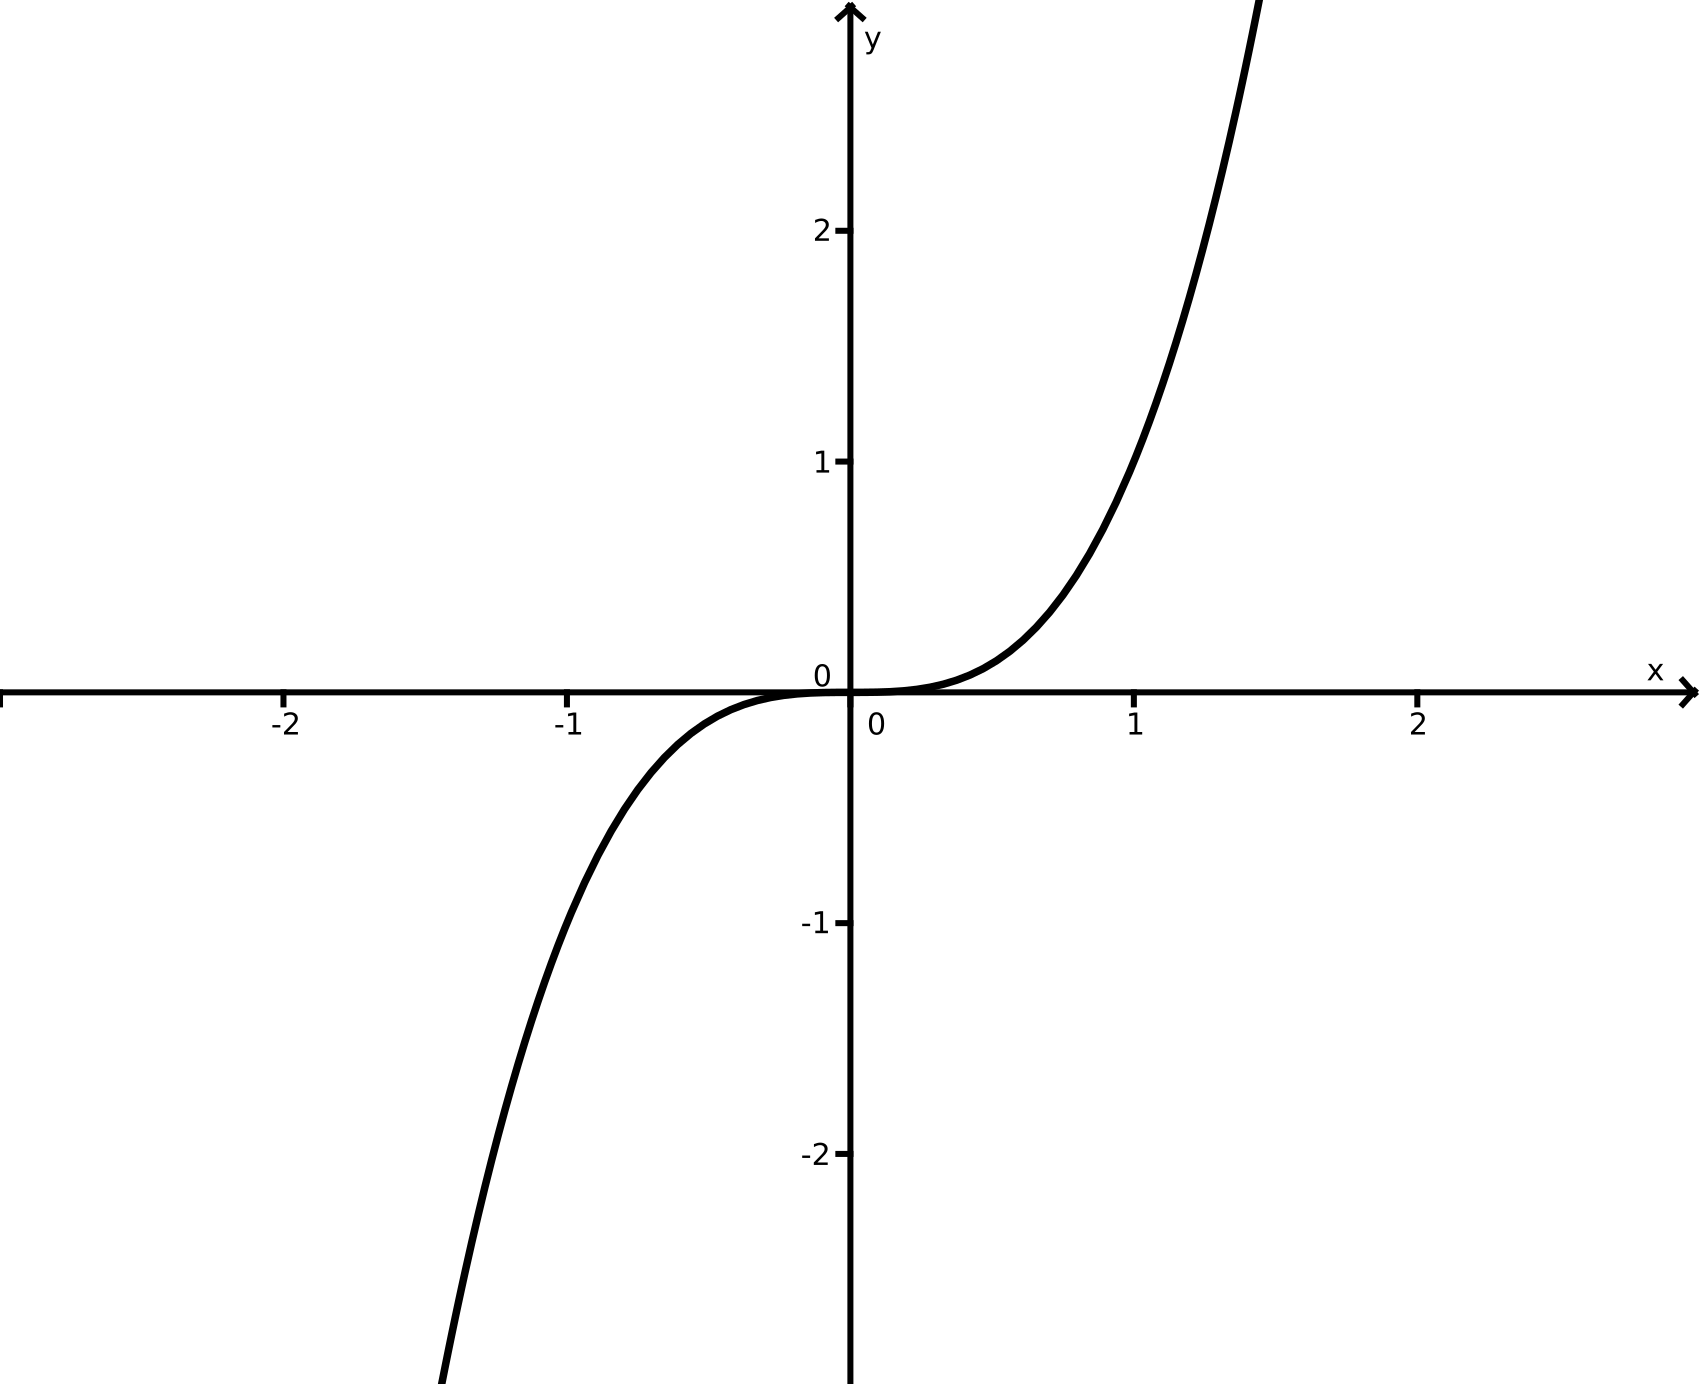
\includegraphics[scale=0.4]{img/2/1}
      \caption{Zeichnung zu 2.}
    \end{figure}    
    
    \item $a>0 \implies \lim_{n\to \infty} a^\frac{1}{n}=1$ Siehe Übung
    
    \item $\lim_{n \to \infty} n^\frac{1}{n}=1$ Siehe Übung 
    
    \item Sei $q\in \R, |q|<1$
    
    $\implies \lim_{n \to \infty} q^n=0$
    
    $\implies \frac{1}{|q|}>1 \implies h:=\frac{1}{|q|}-1>0$
    
    Sei $\epsilon > 0$: Aus Bernoulli: 
    
    $|q|^{-n}=(1+h)^n \geq 1+n \cdot h> n \cdot h>\frac{1}{\epsilon}$
    
    für $n> \frac{1}{\epsilon \cdot h}=:k_\epsilon$
    
    $\implies |q^n-0|=|q^n|=|q|^n < \frac{1}{n \cdot h} < \epsilon$
    
    für alle $n > \frac{1}{\epsilon \cdot h}$
    
    \item $\forall q \in \R, |q|<1,p \in \N$
    
    $\lim_{n \to \infty} n^p \cdot q^n=0$
    
    \textbf{Beweis} O.B.d.A $a \neq 0$
    
    $h := \frac{1}{|q|}-1$
    
    $\implies |q|^{-n} = (1-h)^n = \sum_{k=0}^n \binom{n}{k} h^k$
    
    Sei $\boxed{n>2p} > \binom{n}{p+1} h^k$
    
    $=\frac{n!}{(p+1)!(n-p-1)!} h^{p+1}$
    
    $\underbrace{n \cdot (n-1) \cdot \ldots \cdot (n-p)}_{p+1 \text{ Faktoren}} \cdot \frac{h^{p+1}}{(p+1)!}$
    
    $>\left(\frac{n}{2}\right)^{p+1} \frac{h^{p+1}}{(p+1)!}$
    
    $\implies |p|^n < \left(\frac{2}{h}\right)^{p+1} \frac{(p+1)!}{h^{p+1}}$
    
    $\implies n^p|q|^h < \frac{2^{p+1}(p+1)!}{h^{p+1}} \cdot \frac{1}{n}$
    
    Sei $\epsilon >0$ wähle $k_\epsilon \in \N$,
    
    $k_\epsilon > max\left(2p,\frac{h^{p+1}}{2^{p+1}(p+1)!} \cdot \frac{1}{\epsilon}\right)$
    
    $\implies |n^p \cdot q^n-0|=n^p|q|^n < \epsilon \quad \forall n \geq k_\epsilon$
  \end{enumerate}
\end{example}

\textbf{Notation} Sei $n \in \N$, $A(n)$ Aussagen.

Wir sagen $A(n)$ ist wahr für fast alle $n$, falls $\exists k \in \N: A(n)$ ist wahr $\forall n \geq k$

(Oder: $A(n)$ ist wahr bis auf endlich viele $n$)

\begin{example}
  $\lim a_n = L \Longleftrightarrow \forall \epsilon > 0: |a_n-L|<\epsilon$ für fast alle $n$
  
  $\Longleftrightarrow \forall \epsilon > 0$ sind fast alle $a_n$ in einer $\epsilon$-Umgebung von $L$.
\end{example}

\subsection{Satz 3}

\begin{enumerate}

  \item Sei $(a_n)_n$ eine konvergente Folge, dann ist der Grenzwert eindeutig!
  
    \begin{proof}
    
      \textbf{Angenommen} $a_n \to L$ und $a_n \to R,L\neq R$
      
      \begin{figure}[!ht]
        \centering
          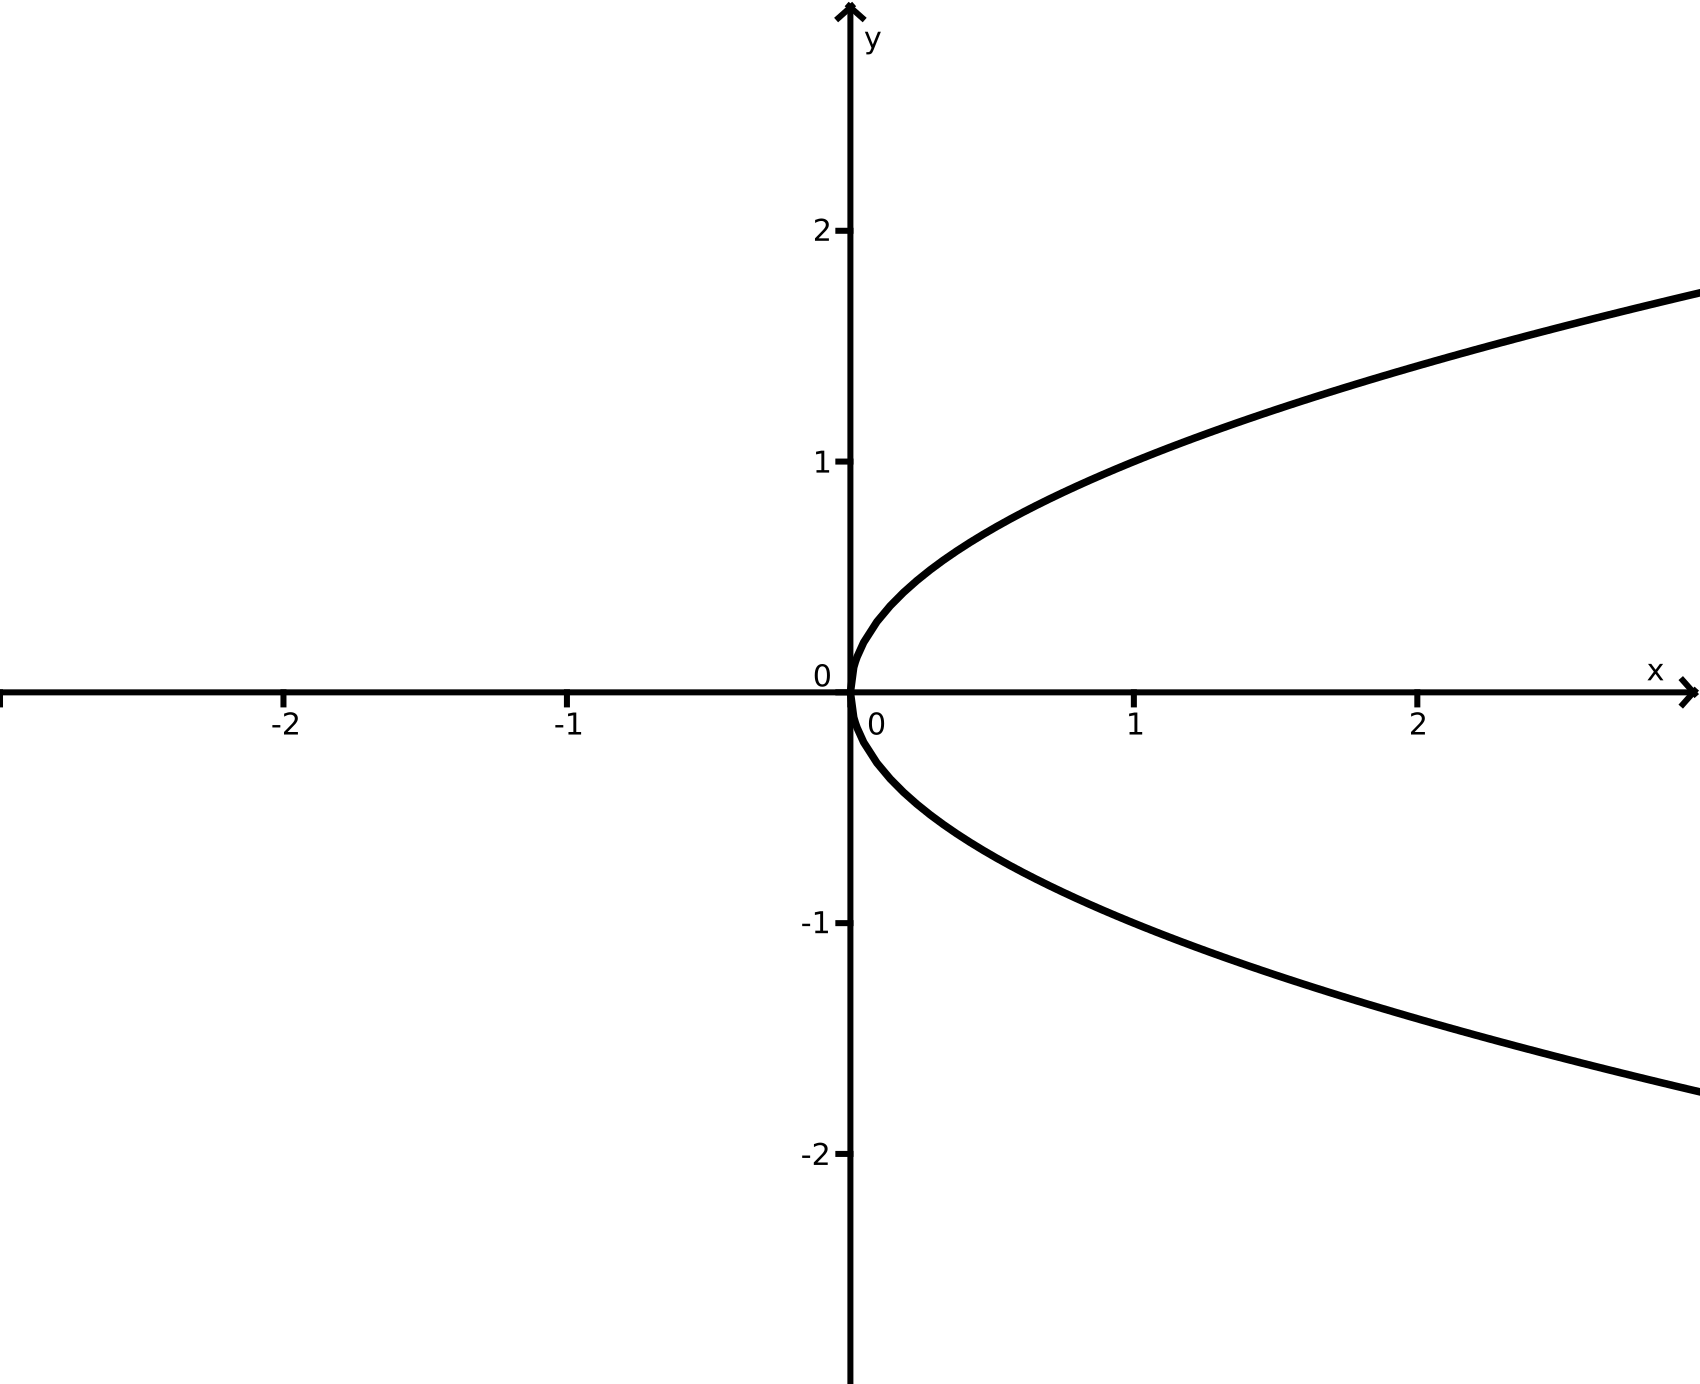
\includegraphics[scale=0.4]{img/2/2}
        \caption{Zeichnung zum Beweis}
      \end{figure}          
      
      $L<R \quad \epsilon := \frac{R-L}{2} >0$
      
      Dann gilt: $\exists k_1 \in \N:|a_n - L|< \epsilon \quad \forall n \geq k_1$
      
      $\exists k_2 : |a_n -R| < \epsilon \quad \forall n \geq k_2$
      
      $\implies n \geq max(k_1,k_2): a_n-L > \epsilon$ und $a_n-R < \epsilon$
      
      $\implies a_n < L+\epsilon = L+\frac{R-L}{2}=\frac{R+L}{2}$
      
      $=R-\epsilon < a_n \lightning$
    \end{proof}  
  
  \item Sei $(a_n)_n$ eine konvergente Folge, dann ist sie beschränkt, d.h. $\exists M \in [0,\infty):|a_n|\leq M \forall n \in \N$
  
  \begin{proof}

    Sei $\epsilon = 1 \implies \exists k_1 \in \N: |a_n -L| < 1$ und $n \geq k_1$
    
    $\implies |a_n| = |a_n-L+L| \leq |a_n -L|+ |L|<|L|+1$
    
    $\implies M:= max(|a_1|,|a_2|,\ldots,|a_{k_1}|,|L|+1)$
    
    $\implies |a_n| \leq M \quad \forall n \in \N!$
    
  \end{proof}
\end{enumerate}

\subsection{Lemma 4}

Sein $(a_n)_n,(b_n)_n$ Folgen

$a_n \to L, a_n-b_n \to 0$ (WORT?!? $a_n-b_n$ ist eine Nullfolge)

\begin{proof}

  Typisches $\frac{\epsilon}{2}$ Argument
  
  \begin{tabular}{rl}
    Sei $\epsilon > 0 \implies$ existiert & $k_1(\epsilon): |a_n-L|<\frac{\epsilon}{2} \quad \forall n \geq k_1(\epsilon)$ \\
    
                                      und & $k_2(\epsilon): |a_n-b_n|<\frac{\epsilon}{2} \quad \forall n \geq k_2(\epsilon)$
  \end{tabular}
  
  Setze: $k(\epsilon):=max(k_1(\epsilon),k_2(\epsilon))$
  
  $|b_n-L| = |b_n-a_n+a_n-L|$
  
  $\leq |b_n -a_n|+|a_n-L|$
  
  $<\frac{\epsilon}{2}+\frac{\epsilon}{2}=\epsilon$
  
  \begin{figure}[!ht]
    \centering
      \includegraphics[scale=0.4]{img/2/3}
    \caption{Zeichnung zum Beweis}
  \end{figure}
 
\end{proof}

\subsection{Satz 5: Rechenregeln für Limes}

Sei $a_n\to a, b_n \to b, \lambda $ eine Zahl.

\begin{enumerate}
  \item $\lim(a_n+b_n)=a+b$
  
    $\lim(\lambda \cdot a_n)=\lambda \cdot a$
    
    $\lim(a_n \cdot b_n)=a \cdot b$
    
    und falls $b \neq 0 \implies b_1 \neq 0$ für fast alle $n$: $\lim \frac{a_n}{b_n} = \frac{a}{b}$ 
 
  \begin{proof}
    
    $\frac{\epsilon}{2}$ Angenommen.
    
    \begin{tabular}{rl}
      Sei $\epsilon > 0$ & $\exists k_1:|a_n-a|<\frac{\epsilon}{2} \quad \forall n \geq k_1$ \\
    
                         & $\exists k_2:|b_n-b|<\frac{\epsilon}{2} \quad \forall n \geq k_2$
    \end{tabular}

    $\implies$ für $n\geq k := \max(k_1,k_2)$ gilt

    $|(a_n+b_n)-(a+b)|=|a_n-a+b_n-b|$
  
    $\leq |a_n-a| + |b_n-b| < \frac{\epsilon}{2}+\frac{\epsilon}{2}= \epsilon$
  
    \textbf{Produkt:} $a_n \cdot b_n-a \cdot b=(a_n-a)b_n+a(b_n-b)$
  
    $=|a_n \cdot b_n -a \cdot b| \leq |a_n-a||b_1|+|a||b_n-b|$
    
    $b_n \to b \implies |b_n|$ ist beschränkt 
    
    d.h. $\exists 0 < M < \infty: |b_1| \leq M \quad \forall n$
    
    \begin{tabular}{rl}
      \textbf{Gegeben} $\epsilon > 0$ Wähle & $k_1: |a_n-a|<\frac{\epsilon}{2M} \quad \forall n \geq k_1$ \\
                                            & $k_2: |b_n-b|<\frac{\epsilon}{2(|a|+1)} \quad \forall n \geq k_2$
    \end{tabular}

	$\implies \forall n > \max(k_1,k_2):$


    \begin{tabular}{rl}
      $|a_nb_n-a \cdot b|$ & $\leq |a_n-a||b_n|+|a||b_n-b|$ \\
                     & $< \frac{\epsilon}{2M}M+|a|\frac{\epsilon}{2(|a|+1)} \leq \epsilon$
    \end{tabular}
    
    \textbf{Quotient} $\frac{a_n}{b_n}=a_n \cdot \frac{1}{b_n}$
    
    d.h. reicht zu zeigen, dass $\frac{1}{b_n} \to \frac{1}{b}$
    
    $b_n \neq 0$ für fast alle $n \quad b \neq 0$
    
    
    $\epsilon = \frac{|b|}{2} \implies |b_n-b|<\frac{|b|}{2}$ für fast alle $n$.
    
    \begin{tabular}{rl}
      $\implies |b_n| =$  & $ |b+b_n-b| \geq |b|-|b_n-b|$  \\
                      $>$ & $ |b| - \frac{|b|}{2}=\frac{|b|}{2}>0$ für fast alle $n$
    \end{tabular}    
    
    $\implies b_n \neq 0$ für fast alle $n$.
    
    $|\frac{1}{b_n}-\frac{1}{b}|=|\frac{b-b_n}{b \cdot b_n}|=\frac{1}{|b||b_n|}|b-b_n| \stackrel{\text{ für fast alle } n}{\leq}\frac{2}{|b|^2}|b_n-b|$

    Da $b_n \to b \implies |b_n-b| < \frac{|b|^2}{2} \epsilon$ für fast alle $n$
    
    $\implies |\frac{1}{b_n}-\frac{1}{b}|\leq \frac{2}{|n|^2}|b_n-b|<\epsilon$ für fast alle $n$

  \end{proof} 
  
  \item $\lim |a_n| = |a|$
  
  \begin{proof}
    Da $||a_n|-|a|| \leq |a_n-a|$ ist er einfach 
  \end{proof}
  
  \item Aus $a_n \leq b_n$ für fast alle $n$ folgt $a \leq b$
  
  Insbesondere: $a_n \geq 0$ für fast alle $n$

  $\implies a \geq 0$
  
  \begin{proof}
  
    Kontraposition $a_n\to a,b_n \to b$
    
    Sei $a>b$
    
    \begin{figure}[!ht]
      \centering
        \includegraphics[scale=0.4]{img/2/4}
      \caption{Zeichnung zum Beweis}
    \end{figure}
    
    Sei $\epsilon = \frac{a-b}{2}>0$
    
    \begin{tabular}{rl}
      $\implies [a_n > a-\epsilon =$ & $ a- \frac{a-b}{2} = \frac{a+b}{2}$ \\
                                $=$ & $b+\frac{a+b}{2}=b+\epsilon>b_n]$
    \end{tabular} 
    
    für fast alle f*cking $n$.    
    
  \end{proof}
    
\end{enumerate}

\subsection{Satz 6} 

\begin{enumerate}
  \item Ist $(a_n)_n$ eine Nullfolge, d.h. $a_n \to 0$ und $(c_n)_n$ beschränkt $\implies (a_n \cdot c_n)_n$ eine Nullfolge.
  
  \begin{proof}
    Es gelte $|c_n| \leq C < \infty$
    
    $b_n := a_nc_n \implies |b_n| \leq C|a_n|$
    
    d.h. 2) $\implies$ 1)    
    
  \end{proof}  
  
  \item Aus $a_n \to 0, |b_n| \leq C|a_n|$ für fast alle $n$ 
  
  ($C$ ist eine Konstante) $\implies b_n \to 0$
  
  \begin{proof}
    Sei $\epsilon > 0$ zu $\epsilon_1 := \frac{\epsilon}{C} \exists k_{\epsilon_1} : |a_n| < \epsilon_1 \forall n \geq k_{\epsilon_1}$
    
    $\implies b_n \to 0$
  \end{proof}
  
\end{enumerate}

\subsection{Satz 7: Sandwich Theorem}

Sei $(a_n)_n$, $(b_n)_n$ konvergente Funktionen 

mit $\lim a_n  = \lim b_n = a$ 

und $(c_n)_n \cdot a_n \leq c_n \leq b_n$ für fast alle $n$

$\implies (c_n)_n$ konvergiert und bei $c_n=a$

\begin{proof}
  Sei $\epsilon > 0$
  
  $\exists k_1: a_n \leq c_n \leq b_n \quad \forall n \geq k_1$
 
  $\exists k_2: |a_n-a|<\epsilon \quad \forall n \geq k_2$
  
  $\exists k_3: |b_n-a|<\epsilon \quad \forall n \geq k_3$
  
  $\implies \forall n \geq \max(k_1,k_2,k_3)$

  $a-\epsilon < a_n \leq c_n \leq b_n < a+\epsilon$

  d.h. $|c_n -a| \leq \epsilon$  
  
\end{proof}

\begin{example}

  \begin{itemize}
    \item $\forall p \N: \lim_{n\to \infty} (n^p)^{\frac{1}{n}}=1$
    
    \begin{proof}
      \begin{itemize}
        \item $p=1:$ Übung!
        
        \item $p=2: \lim(n^2)^{\frac{1}{n}} = \lim(n^{\frac{1}{n}} \cdot n^{\frac{1}{n}})$
        
          $= \lim_{n \to \infty} n^{\frac{1}{n}} \cdot  \lim_{n \to \infty} n^{\frac{1}{n}}$ 

	      $1 \cdot 1=1$
	    \item $p \geq 2$ Induktionsbeweis
      \end{itemize}
    \end{proof}
    \item $\lim \frac{a \cdot n+b}{c \cdot n+a} = \frac{a}{c}$ falls $c\neq 0$
    
    \begin{proof}
      $\frac{a \cdot n+b}{c \cdot n+a} = \frac{a+\frac{b}{n}}{c+\frac{d}{n}} \stackrel{\text{ Quotientenregel }}{\to} \frac{a}{c}$
    \end{proof}
        
    $\lim_{n\to \infty} \frac{a \cdot n+d}{c \cdot n^2+d \cdot n+f}\neq \stackrel{c \neq 0 }{0}$
    
    \begin{proof}
      $\frac{a \cdot n+d}{c \cdot n^2+d \cdot n+f}= \frac{1}{n} \cdot \frac{a+\frac{d}{n}}{c+\frac{d}{n}+\frac{f}{n^2}} \to \stackrel{c\neq 0}{0}$
    \end{proof}
  \end{itemize}

\end{example}

\section{Divergente Folge}
\subsection{Definition 8} Eine Folge $(a_n)_{n \in \N}$ heißt bestimmt divergent gegen $\infty$ (bzw. $-\infty$), in Zeichen, $\lim_{n\rightarrow \infty} = \infty, a_n \rightarrow \infty$ (bzw. $\lim_{n\rightarrow\infty} a_n = - \infty , a_n \rightarrow - \infty$) falls $\forall k > 0 \exists N = N(k): a_n > k \forall n \geq N$ (bzw. $a_n < -k \forall n \geq N$)\\
z.B. $a_n = n, a_n = n^2$
\subsection{Rechenregeln} Die regeln von S4 gelten sofern die rechten Seiten Definiert sind.\\
z.B. $a_n = n, b_n = n^2 \implies a_n + b_n \rightarrow \infty + \infty = \infty$, also $a_n - b_n \rightarrow \infty - \infty$ nicht definiert\\
$n - n^2 = (\frac{1}{n} - 1) n^2 \leq -\frac{1}{2}n^2, n\geq 2 \rightarrow \infty$\\
insb gilt:
\begin{enumerate}[1)]
\item $a_n \rightarrow \infty \implies \lambda a_n \rightarrow \infty$ für $\lambda > 0, \lambda a_n \rightarrow - \infty, \lambda < 0$
\item $a_n \rightarrow \infty \rightarrow \frac{1}{a_n} \rightarrow 0$ und falls $a_n > 0$ für fast alle n, dann gilt auch Umkehrung
\item $a_n \rightarrow \infty, b_n \rightarrow b \in \R \implies a_n + b_n \rightarrow \infty$
\item $a_n \rightarrow \infty, b_n \rightarrow b > 0$ (oder $b_n \rightarrow \infty$) $\implies a_n  \cdot  b_n \rightarrow \infty$
\end{enumerate}
\begin{proof}
\begin{itemize}
\item 1) - 3): Scharf hinschauen
\item 4) $b_n \rightarrow b > 0 \implies b_n \geq \frac{1}{2} b$ für fast alle n, $\implies a_n  \cdot  b_n > \frac{1}{2}b \cdot a_n$ für fast alle n.\\zu $k > 0$, wähle $N(k): a_n > \frac{2}{b}k \forall n\geq N(k)$\\$\implies a_n  \cdot  b_n > \frac{b}{2}  \cdot  \frac{2}{b} k = k$ für fast alle n
\end{itemize}
\end{proof}
\section{Monotone Folgen}
\subsection{Definition 9} Eine Folge $(a_n)_n$ reeller Zahlen heißt
\begin{enumerate}[1)]
\item wachsend, falls $a_n \leq a_{n+1} \forall n \in \N$
\item fallend, falls $a_n \geq a_{n+1} \forall n \in \N$
\item monoton, falls sie wachsend oder fallend ist.
\end{enumerate}
\subsection{Satz 10 (Monotone Konvergenz)} Jede beschränkte monotone Folge ist konvergen! Insb:
\begin{enumerate}[1)]
\item $(a_n)_n$ wachsend (beschränkt) $\implies \lim_{n\rightarrow\infty} a_n = \sup_{n\in\N}a_n$
\item $(a_n)_n$ fallend (beschränkt) $\implies \lim_{n\rightarrow \infty} a_n = \inf_{n\in\N}a_n$
\end{enumerate}
\begin{proof}
\begin{enumerate}[1)]
\item Sei $a:=\sup a_n = \sup \{a_n: n\in\N\}\in\R$ wegen Vollständigkeitsaxiom

Sei $a>0$. Nach Definition von Supremum $\exists k_\epsilon \in \N$

$\alpha - \epsilon < a_{k_\epsilon} \leq a_{k-{\epsilon + 1}} \leq ... \leq a_n \leq \alpha \forall n \leq k_\epsilon$
\item Wende 1) auf $b_n = -a_n a_n$
\end{enumerate}
\end{proof}
\subsection{Korollar 11} Sei $(b_n)_n$ Folge mit $\frac{|b{n+1}|}{|b_n|} \rightarrow x$ für $o \leq x < 1 \implies \lim b_n = 0$\\insb. $\lim q^n = 0, |q|<1$

\begin{proof}
Z.z. $|b_n| \rightarrow 0$ d.h. O.B.d.A. $b_n > 0$. Da $\frac{b_{n+1}}{b_n} \rightarrow x$ für $0 \leq x < 1$

Wähle $s = 1 -x > 0 \implies \exists N$

$\frac{b_{n+1}}{b_n} < x + \epsilon = 1 \forall n \geq N$

$\implies b_{n+1} < b_n \forall n \geq N$

$\implies L = \lim_{n \rightarrow \infty} b_n$ existiert und $L \geq 0$. Wollen $L = 0$

\subsubsection{Angenommen:} $L>0$

$\implies [x = \lim \frac{b_{n+1}}{b_n} \underbrace{=}_{\text{Quotientenmenge}} \frac{\lim b_{n+1}}{\lim b_n} = \frac{L}{L} = 1] \lightning$ d.h. $L = 0$!
\end{proof}

\subsection{Korollar 12 (Rekursive Berechnung von \texorpdfstring{$\sqrt{a}$}{Wurzel a}} 
Sei $a > 0, x_0 > 0$. Definiere $(x_n)_{n\in\N}, x_{n+1} := \frac{1}{2} (x_n+ \frac{a}{x_n}) | n\in\N$. 
Dann konvergiert $x_n, \lim x_n = \sqrt{a}, x_n > 0 \forall n$

\begin{proof}
Per Induktion zeigt man $x_n > 0 \forall n$
\end{proof}
\begin{enumerate}[\text{Fakt }1:]
  \item $x_n \geq \sqrt{a} \forall n > 1,$ da $x_{n+1}^2 -a = \frac{1}{4}(x_n - \frac{a}{x_n})^2 - a$\\
    $= \frac{1}{4}(x_n^2 - 2a + \frac{a^2}{x_n^2}  4a)$\\
    $= \frac{1}{4}(x_n-\frac{a}{x_n})^2 \geq 0$
  \item Für $n \geq 1$ ist $(x_n)_n$ fallend, da 
    $$x_n - x_{n+1} = x_n - \frac{1}{2} (x_n + \frac{a}{x_n}) = \frac{1}{2}(x_n - \frac{a}{x_n})$$
    $=\underbrace{\frac{1}{2x_n}}_{\geq 0} \underbrace{(x_n^2 -a}_{\geq 0} \geq 0$ wegen Fakt 1) \\
    $\implies \lim_{n \rightarrow \infty} x_n = x$ existiert $\geq \sqrt{a}$\\
    $\implies x = \lim x_{n+1} = \frac{1}{2} \lim (x_n + \frac{a}{x_n} = \frac{1}{2} (x + \frac{a}{x})$\\
    $\implies x^2 = a$, da $x > 0 \implies x = \sqrt{a}$

\begin{proof}
$$f_n := x_n - \sqrt{a} \implies f_{n+1} = x_{n+1} - \sqrt{a} = \frac{1}{2}(x_n + \frac{a}{x_n}) - \sqrt{a}$$
$$= \frac{1}{2x_n}(x_n^2 -a) - \sqrt{a} = \frac{1}{2x_n}(x_n - \sqrt{a})^2 = \frac{f_n^2}{2x_n} \leq \frac{1}{2\sqrt{a}} f_n^2$$, $n\geq 1$
quadratische Konvergenz
\end{proof}
\end{enumerate}

\subsection{Korollar 13}
$e := \lim_{n \rightarrow \infty} (1 + \frac{1}{n})^n$ existiert und $2 + \frac{1}{3} < e \leq \frac{6^7}{2n} < 2,78167$

\begin{proof}
\[a_n = (1 + \frac{1}{n})^n \implies a_n\text{ ist wachsend da } n\geq 2\]
\[\frac{a_n}{a_{n-1}} = \frac{(1+\frac{1}{n})^n}{(1+\frac{1}{n-1})^{n-1}} = \frac{(\frac{n+1}{n})^n}{(\frac{n}{n-1})^{n-1}}\]
\[= \frac{n}{n-1}  \cdot  (\frac{(n+1)(n-1)}{n^2})^n = \frac{n}{n-1} (\frac{n^2 - 1}{n^2})^n\]
\[= \frac{n}{n-1} (1-\frac{1}{n^2})^n \underbrace{>}_{\text{Bernoulli}} \frac{n}{n-1} (1 - n  \cdot  \frac{1}{n^2}) = 1\]
Monotone Konvergenz $\implies a_n$ konvergiert, wenn es nach oben beschränkt ist.
\[a_n = (1 + \frac{1}{n})^n = \sum_{k = 0}^n \binom{n}{k} (\frac{1}{n})^k = \sum_{k=0}^n \frac{n!}{k!(n-k)!}  \cdot  \frac{1}{n^k}\]
\[= \sum_{k =0}^n \frac{1}{k!} \prod_{l=0}^k \frac{n-l}{n} \leq \sum_{k=0}^n \frac{1}{k!}\]
Induktion $=: k! \geq 2^k$ für $k\geq 4$
\[\implies n \geq k: a_n \leq 1 + 1 + \frac{1}{2} +  \frac{1}{2  \cdot  3} + \sum_{k = 4}^n (\frac{1}{2})^k\]
\[= \frac{16}{6} + \frac{1}{2^4} \sum_{l = 0}^{n-4} (\frac{1}{2})^l = \frac{16}{6} + \frac{1}{2^4} \underbrace{(\frac{1-(\frac{1}{2})^{n-3}}{1-\frac{1}{2}})}_{\leq 2} \text{(geometrische Summe)}\]
\[\leq \frac{16}{6} + \frac{1}{8} = \frac{67}{24} \implies e \leq \frac{67}{24}\]
\[e \geq a_n \forall n, n = 3\]
\[=(1 + \frac{1}{2})^k, e \geq a_3 = 2 + \frac{10}{27} > 2 + \frac{1}{3}\]
\end{proof}
\section{Teilfolgen und Häufungswerte}
\subsection{Definition 14: (Teilfolgen, Umordnung)} $(a_n)_n$ Folge $a = (a_n)_{n}: \N \rightarrow \R$\\
$\phi : \N \rightarrow \N$ bijektiv\\
$\implies b:= a \circ \phi$, d.h. $b = (b_l)_{l\in\N}$, $b_l := a_{\phi (l)}$\\
b : Umordnung von $(a_n)_n$\\
Wir nennen $\sigma : \N \rightarrow \N$ eine Verdünnung falls $\sigma$ strikt monoton steigend ist, d.h. $\sigma (n) < \sigma (n+1) \forall n$. Dann ist $(b_l)_l$ definiert durch $b_l := a_{\sigma (l)}$ eine Teilfolge von $(an)_n$
\subsubsection{Bemerkung:}
\begin{enumerate}[1)]
\item Für jede Verdünnung $\sigma$ gilt $\sigma (n) \geq n \forall n \in \N$ (Warum?)
\item $(a_n)_n := (\frac{1}{n})_n$, $(\frac{1}{2n})_n$, $(\frac{1}{n^2})_n$ sind Teilfolgen von $(a_n)_n$\\
$\sigma(n) = 2n$, $b_{\sigma(l)} = a_{2l} = \frac{1}{2l}$\\
$\sigma(n) = n^2$, $b_n = a_{\sigma(n)} = a_n^2 = \frac{1}{n^2}$\\
$(\frac{1}{2}, 1, \frac{1}{4}, \frac{1}{3}, \ldots$ ist eine Umordnung von $(1, \frac{1}{2}, \frac{1}{3}, \frac{1}{4}, \ldots)$
\end{enumerate}
\subsection{Lemma 15} Jede Umordnung und jede Teilmenge einer konvergenten Folge konvergiert mit demselben Grenzwert! Und dasselbe gilt, wenn man endlich viele Werte von $a_n$ abändert.

\begin{proof}
Für Umordnung nachrechnen.\\
Sei $b_n = a_{\sigma(n)}$ Teilfolge von $(a_n)_n$\\
$a_n \rightarrow L : \forall \epsilon > 0 : \exists k_\epsilon: |a_n - L| < \epsilon : \forall n \geq k_\epsilon$\\
Da $\sigma(n) \geq n \forall n \in \N$ gilt auch $\forall n \geq k_\epsilon \implies \sigma(n) \geq k_\epsilon $  \\
$|b_n - L| = |a_{\sigma(n)} - L| < \epsilon$
\end{proof}
\subsection{Definition 16 Häufungswert}
Sei $(a_n)_n$ eine Folge, $a\in\R$ ist ein Häufungswert von $(a_n)_n$, falls $\forall \epsilon > 0$ gibt unendlich viele $n\in\N$ mit $|a_n - a| < \epsilon$
\subsubsection{Beispiel} 
\begin{enumerate}
\item $a_n = \frac{1}{n}$ hat Häufungswert 0

\item $a_n = (-1)^n$ hat Häufungswert 1 und -1

\item $a_n = (-1)^n + \frac{1}{n}$ hat HW 1 und -1

\end{enumerate}

$H((a_n)_n) = $ Menge der HW von $(a_n)_n = \{ a\in\R$, $a$ ist HW von $(a_n)_n\}$
\subsubsection{Bemerkung}
\begin{enumerate}[1)]
\item Für eine beschränkte Folge $(a_n)_n$ gilt: $$a_n \rightarrow a \Leftrightarrow H((a_n)_n) = \{a\}$$
\item $(n)_{n\in\N}$ hat keinen Häufungswert!
\end{enumerate}
\subsection{Satz 17 (Bolzano - Weierstraß für Folgen)} Jede beschränkte Folge hat mindestens einen HW

\begin{proof}
Sei $(a_n)_n$ beschränkt, z.B. $c \leq a_n \leq d \forall n$\\
$G := \{ x\in\R: a > x$ für höchstens endlich vielen$\}$\\
$=\{x\in\R: a_n \leq x$ für fast alle n$\}$
\begin{enumerate}[\text{Fakt }1)]
\item $G \neq \emptyset$, da $d \in G$
\item $G$ ist nach unten beschränkt, denn $x \notin G$, falls $x < c \implies \alpha := \inf G \in \R$

\subsubsection{Behauptung} $\alpha \in H((a_n)_n)$\\
Dann sei $\epsilon > 0 \implies$ nach Definition von Infimum \\
$\alpha + \epsilon \in G$ und $\alpha - \epsilon \notin G$ \\
$\implies$ fast alle $a_n < \alpha + \epsilon$ und unendlich viele $a_n > \alpha - \epsilon$\\
$\implies$ Es gibt unendlich viele $n: |a_n - \alpha| < \epsilon \implies \alpha \text{ ist Häufungswert}$
\end{enumerate}
\end{proof}

\subsection{Lemma 18} 
(\textbf{Erinnerung:} $h$ Häufungswert von $(a_n)_n$ falls $\forall \epsilon > 0 $. $a_n \in B_\epsilon (h):= (h-\epsilon, h+\epsilon)$ für unendlich viele $n \in \N$)

Sei $(a_n)_n $ Folge

$h \in H((a_n)_n) \Longleftrightarrow \exists$ Teilfolge von $(a_n)_n$ die gegen $h$ konvergiert.

\begin{proof}
  \[\mqq{\Longleftarrow}: \text{ ist } (a_{n_j})_j, n_j < n_{j+1} \quad \forall j\]
  \[\text{Teilfolgen } (a_n)_n \text{ mit } \]
  \[ \lim_{j \to \infty} a_{h_j} = h\]
  \[\text{dann sind für } \epsilon > 0 \text{ fast alle } a_{n_j} \in B_\epsilon(h)\]
  \[\implies \exists \text{ unendlich viele } n: a_n \in B_\epsilon(h)\]
  \[\implies h \text{ ist Häufungswert } \surd \]
  \[\mqq{\Longrightarrow}: h \in H((a_n)_n) \text{ d.h. }\]
  \[\underline{\forall \epsilon> 0} \exists \text{ unendlich viele } n: a_n \in B_\epsilon(h)\]
  \[\text{ \underline{Trick:} Wähle } \epsilon= \frac{1}{l}, l \in \N\]
  \[\forall l \in \N: \exists \text{ unendlich viele } n: a_n \in B_\frac{1}{l}(h)\]
  \[\text{rekursive Definition der Teilfolge}\]
  \[
    \begin{array}{ll}
      n_1 & := \text{ ersten } n \in \N: a_n \in B_1(h) \\
          & := \min\left\{n \in \N: a_n \in B_1(h) \right\}
    \end{array}
  \]
  \[
    \begin{array}{ll}
      n_2 & := \text{ ersten } n \in \N, n > n_1, a_n \in B_\frac{1}{2}(h) \\
          & := \min\left\{n \in \N, n > n_1, a_n \in B_\frac{1}{2}(h) \right\}
    \end{array}
  \]
  \[\ldots\]
  \[n_{j+1}:= \min\left\{n \in \N, n > n_j, a_n \in B_\frac{1}{j+1}(h)\right\}\]
  \[\text{ nachrechnen: } \boxed{n_l < n_{l+1}} \quad \forall l\]
  \[a_{n_l} \in B_\frac{1}{l}(h) \implies \lim_{l \to \infty} a_{n_l} = h\]
  \[(b_l)_l, b_l = a_{n_l} \text{ ist Teilfolge von } (a_n)_n\]
\end{proof}

\subsection{Korollar 9: Balzano-Weierstraß für Folgen II}

Jede beschränkte Folge hat eine konvergente Teilfolge! (Beweis S.17 + L.18).

\section{Asymptotisches Verhalten von reellen Folgen (\texorpdfstring{$\limsup$}{Limes superior} und \texorpdfstring{$\liminf$}{Limes inferior})}


\textbf{Frage:} Gibt es unter allen Häufungswerten einen größten bzw. kleinsten?
\[(a_n)_n \text{ beschränkt: } \sup_{n \in \N} a_n \in \R, \inf_{n \in \N} a_n \in \R \]
\[\Longrightarrow H((a_n)_n) \subset \left[\inf_{n \in \N} a_n,\sup_{n \in \N} a_n \right] \]

\begin{example}
\[a_1:= 10^{10^{10}}\]
\[a_2:= -10^{10^{10}}\]
\[a_n:= 0 \quad n\geq 3\]

\[\left[ -10^{10^{10}}, 10^{10^{10}} \right] \subset H((a_n)_n)=\{0\}\]
Eigentlich interessiert uns $n$ groß!
\end{example}
\[ b_l := \sup_{n \geq l} a_n \]
\[ c_l := \inf_{n \geq l} a_n \]

\begin{enumerate}
 \item $\boxed{c_l \leq b_l \quad \forall l} $
   \[
     \begin{array}{ll}
       \text{und } & b_{l+1} \leq b_l \forall \text{ fallend} \\
                    & c_{l+1} \geq c_l \forall \text{ wachsend} 
     \end{array}
   \]
   \[\text{ist } (a_n)_n \text{ beschränkt } \implies (b_l)_l, (c_l)_l \text{ beschränkt }\]
   \[\stackrel{\text{monotone Konvergenz}}{\implies} \lim_{l\to \infty} b_l \geq \lim_{l \to \infty} c_l\]
   \[\text{existieren!}\]
 \item $ \forall \epsilon > 0 \forall l \in \N $ sind fast alle $\begin{array}{c}a_n<b_l+\epsilon \\ a_n > c_l -\epsilon \end{array}$
\end{enumerate}

\subsection{Definition 20}

Sei $(a_n)_n$ reelle Folge 
\[\limsup_{n \to \infty} a_n:= \overline{\lim_{n \to \infty}} a_n:= \overbrace{\lim_{l \to \infty} \left(\sup_{n \geq l} a_n\right)}^{=\lim_{l \to \infty} b_l}\]
\[\liminf_{n \to \infty} a_n:= \underline{\lim_{n \to \infty}} a_n:= \underbrace{\lim_{l \to \infty} \left(\inf_{n \geq l} a_n\right)}_{=\lim_{l \to \infty} c_l}\]

Falls $(a_n)_n$ nach oben unbeschränkt ist:
\[\limsup_{n \to \infty} a_n:= +\infty\]
Falls $(a_n)_n$ nach unten unbeschränkt ist:
\[\liminf_{n \to \infty} a_n:= -\infty\]

\underline{Bemerkung} Es gilt
\[\limsup_{n \to \infty} (-a_n) = - \liminf_{n \to \infty}(a_n) \]
\[\liminf_{n \to \infty} (-a_n) = - \limsup_{n \to \infty}(a_n) \]

\[\liminf_{n \to \infty} (a_n) \leq \limsup_{n \to \infty} (a_n)\]

\subsection{Satz 21}

Sei $(a_n)_n$ beschränkte Folge
\[\Longrightarrow \limsup_{n \to \infty} (a_n) \text{ ist der größte Häufungswert von } (a_n)_n\]
und
\[\Longrightarrow \liminf_{n \to \infty} (a_n) \text{ ist der kleinste Häufungswert von } (a_n)_n\]

\begin{proof}

Wegen den Bemerkung reicht es das Erste zu zeigen!
\[\alpha := \limsup_{n \to \infty} (a_n)=\sup(H((a_n)_n))\]

\subsubsection{Schritt 1}
$\forall \epsilon > 0$, gibt es nur endlich viele $n$ mit $a_n> \alpha + \epsilon$
\[\sup_{n \subset \N} a_n = \sup\{a_n:n \in \N\}\]
\begin{proof}
  \[ \text{Sei } \epsilon>0,\quad b_l := \sup_{n \geq l} a_n \text{ ist fallend},\quad b_l \to \alpha\]
  \[\implies \exists l \in \N: b_l < \alpha + \epsilon\]
  \[\Longleftrightarrow \sup_{n \geq l} a_n < \alpha + \epsilon\]
  \[\Longleftrightarrow \text{Höchstens die ersten } l-1 \text{ Glieder von } (a_n)_n \text{ sind } \geq \alpha + \epsilon \]
\end{proof}

\subsubsection{Schritt 2}
$\forall \epsilon > 0$, gibt es unendlich viele $n$ mit $a_n> \alpha - \epsilon$

\begin{proof}
\[\text{Da } b_l:= \sup_{n \geq l} a_n \text{ fallend}\]
\[\implies b_1 \geq b_{l+1} \geq b_{l+2} \geq \ldots \geq b_{l+k} \stackrel{k\to \infty}{\to} \alpha\]
\[\implies b_l \geq \alpha \quad \forall l\]
Sei $\epsilon >0$, $l\in \N$. Aus Definition von Supremum folgt
\[\exists n = n_l \geq l: a_{n_l}>b_l-\epsilon \geq b_{l+1}-\epsilon \geq \ldots \geq b_{l+k}-\epsilon \stackrel{k\to \infty}{\to} \alpha -\epsilon\]
\[\implies \exists n = n_l \geq l: a_{n_l}>\alpha-\epsilon \]
\[\implies \exists \text{ unendlich viele } n: a_n > \alpha - \epsilon!\]
\end{proof}

\end{proof}

\textbf{Bemerkung}

\begin{enumerate}
  \item Also gilt
    \[H((a_n)_n) \subset [\liminf_{n \to \infty} (a_n),\limsup_{n \to \infty} (a_n)] \text{ und } (a_n)_n \text{ konvergent } \]
    \[\Longleftrightarrow \liminf_{n \to \infty} (a_n)\geq\limsup_{n \to \infty} (a_n)\]
    und in \underline{diesem} Fall gilt
    \[\lim_{n \to \infty} (a_n) = \liminf_{n \to \infty} (a_n) = \limsup_{n \to \infty} (a_n)\]
    insbesondere $(c_n)_n$ Nullfolge
    \[\Longleftrightarrow \limsup_{n \to \infty} |c_n| = 0\]
  \item Für 2 Folgen $(c_n)_n$, $(d_n)_n$ gilt
    \[\limsup_{n \to \infty}(c_n+d_n) \leq \limsup_{n \to \infty}(c_n)+\limsup_{n \to \infty}(d_n)\]
    \[\liminf_{n \to \infty}(c_n+d_n) \geq \liminf_{n \to \infty}(c_n)+\liminf_{n \to \infty}(d_n)\]
    \underline{Beispiel} $c_n=(-1)^n,d_n=-(-1)^n$
\end{enumerate}

\section{Das Cauchy-Kriterium für Konvergenz}

\textbf{Bemerkung} Falls $(a_n)_n$ konvergiert:
\[\implies \forall \epsilon > 0 \exists N_\epsilon: |a_n-a_m|<\epsilon \quad \forall n,m \geq N_\epsilon\]
\[(\Longleftrightarrow \forall \epsilon > 0 \exists N_\epsilon: |a_n-a_m|\leq \epsilon \quad \forall n,m \geq N_\epsilon)\]

Deswegen aus $a_n \to L \quad \forall \epsilon > 0 \exists N_\epsilon : |a_n-L|<\frac{\epsilon}{2} \forall n \geq N_\epsilon$
\[\implies |a_n-a_m| \leq |a_n-L|+|L-a_m| < \frac{\epsilon}{2} + \frac{\epsilon}{2} = \epsilon \quad \forall n,m \geq N_\epsilon\]

\textbf{Definition} Eine Folge $(a_n)_n$ heißt Cauchy (oder Cauchyfolge) falls gilt:
\[\forall \epsilon > 0 \exists N_\epsilon: |a_n-a_m|<\epsilon \quad \forall n,m \geq N_\epsilon\]

\textbf{Bemerkung} Eine Folge $(a_n)_n$ ist Cauchy
\[\Longleftrightarrow \limsup_{n,m\to \infty}|a_n-a_m|=0\]
\[\text{wobei } \limsup_{n,m\to \infty}(b_{n,m}):=\lim_{l \to \infty}(\sup_{n,m\geq l}(b_{n,m}))\]

\textbf{Scharfes Hinsehen}

\subsection{Satz 23: Cauchy Kriterium}

Eine Folge $(a_n)_n$ konvergiert $\Longleftrightarrow$ $(a_n)_n$ ist eine Cauchyfolge

\textbf{Vorbereitung:} %Wow, eimal mehr geile Struktur ...%

\subsection{Lemma 24}

Eine Cauchyfolge $(a_n)_n$ konvergiert

\[\Longleftrightarrow (a_n)_n hat eine konvergente Teilfolge\]
\[(\Longleftrightarrow H((a_n)_n) \neq \emptyset )\]

\begin{proof}
  \[\mqq{\Longrightarrow}: \text{ klar}\]
  \[\mqq{\Longleftarrow}: \text{ Sei } (a_{n_l})_l \text{ konvergente Teilfolge von } (a_n)_n\]
  \[\text{d.h.: } n_l < n_{l+1} \quad \forall l \in \N,n\in \N\]
  \[L:= \lim_{n \to \infty} a_{n_l}\]
  Sei $\epsilon > 0$ Da $(a_n)_n$ Cauchyfolge ist
  \[\implies \exists N_\epsilon: |a_n-a_m| < \epsilon \quad \forall n,m \leq N_\epsilon\]
  \fbox{%
    \parbox{0.8\linewidth}{%
  \[\implies \forall n \geq N_\epsilon: \text{ Wähle } m=n_l\geq l, l \geq N_\epsilon\]
  \[\implies \boxed{|a_n-a_{n_l}|} < \epsilon \quad \forall l \geq N_\epsilon\]
        }%
  }
  \begin{align*}
    |a_n-L| & = \lim_{l \to \infty}|a_n-a_{n_l}| \\
            & \leq \limsup_{l \to \infty}\underbrace{|a_n-a_{n_l}|}_{<\epsilon \quad \substack{\forall l\geq N_\epsilon\\n\geq N_\epsilon}} \\
            & \leq \epsilon \quad \forall n \geq N_\epsilon
  \end{align*}

  \[\text{d.h. } a_n \to L!\]

\textbf{oder etwas anders}

  \[|a_n-L| \leq |a_n-a_{n_l}|+|a_{n_l}-L|\]
  \begin{align*}
    \implies |a_n-L| & = \limsup_{l\to\infty}|a_n-L| \\
                     & \leq \limsup_{l\to\infty}\left(|a_n-a_{n_l}|+|a_{n_l}-L|\right) \\
                     & \leq \limsup_{l\to\infty}\underbrace{|a_n-a_{n_l}|}_{<\epsilon}+\underbrace{\limsup_{l \to \infty} |a_{n_l}-L|}_{=0} \\
                     & \leq \epsilon \quad \forall n \geq N_\epsilon
  \end{align*}
\end{proof}

\subsection{Lemma 25: Jede Chauchyfolge ist beschränkt}

\begin{proof}

Sei $\epsilon = 1, \exists N: |a_n-a_m|<1 \quad \forall n,m \geq N$
\[\implies \forall n \geq N : |a_n-a_N|<1\]
\begin{align*}
  \implies \forall n \geq N : |a_n| & \leq |a_n-a_N|+|a_N| \\
                                    & \leq 1+|a_N|
\end{align*}
\[M:= \max(|a_1|,|a_2|,\ldots,|a_N|,1+|a_N|)\]
\[\implies \forall n \in \N: |a_n|\leq M\]
\end{proof}

\begin{proof} von S.23

\[\mqq{\Longrightarrow}:\]
\begin{align*}
  \mqq{\Longleftarrow}: & \text{Sei } (a_n)_n \text{Cauchy} \\ 
                        & \mqq{\stackrel{L.25}{\Longleftarrow}}: (a_n)_n \text{ist beschränkt} \\ 
                        & \mqq{\stackrel{Kor.19}{\Longleftarrow}}: (a_n)_n \text{hat eine konvergente Teilfolge} \\
                        & \implies (a_n)_n \text{ ist Konvergent}
\end{align*}



\end{proof}

\section{Einschub Komplexe Zahlen}

\textbf{Wiederholen} $x^2+1=0$ hat keine Lösung in $\R$ da $\forall x \in \R: x^2 \geq 0$

\textbf{Möchten} $\boxed{\text{Zahl } i, \quad i^2=-1}!$ (imaginäre Zahl)

\textbf{Informel} Schreiben $\begin{array}{lll}z&=a+ib&\quad \boxed{a,b \in \R}\\&=x+iy&\quad \boxed{x,y \in \R}\end{array}$

Man nennt $x$ den Realteil von $z=x+iy$

Man nennt $y$ den Imaginärteil von $z=x+iy$

reelle Zahl $z=x=x+i \cdot 0$

Wollen rechnen: D.h. alle Körperaxiome sollen gelten.

\begin{itemize}
 %\item What does the + say???
 \item Was ist \qq{$+$} (Plus, addieren) ?
 \item Was ist \qq{$ \cdot $} (Mal, multiplizieren) ?
\end{itemize}

\subsection{Summe:} $$z_1 = a_1 + ib_1 \text{, } z_2 = a_2 + ib_2$$ $$\implies z_1 + z_2 := (a_1 + ib_1) + (a_2+ib_2)$$ $$(a_1 + ib_1) + (a_2+ib_2) = (a_1 + a_2) + i(b_1+b_2)$$

\subsection{Produkt:} $$z_1  \cdot  z_2 = (a_1 + ib_1)  \cdot  (a_2  \cdot  ib_2)$$ 
%unsure code
$$=a_1(a_2 + ib_2) + ib_2(a_1)$$
$$a_1a_2 + ia_1b_2 + ia_2b_1 + \underbrace{(ib_1)(ib_2)}_{-b_1 \cdot b_2}$$
$$=a_1a_2 -b_1b_2 + i(a_1b_2 + a_2b_1)$$

\subsection{Definition von Komplexe Zahlen}
$\mathbb{C} := \R \times \R = \R^2=\{\binom{x}{y}:x,y \in \R\}$\\
Mit den binären Operationen:
\begin{itemize}
\item \qq{$+$} $\mathbb{C} \times \mathbb{C} \rightarrow \mathbb{C}$\\ $z_1 = \binom{a_1}{b_1}$ $z_2 = \binom{a_2}{b_2}$\\ $(z_1, z_2) \mapsto z_1 + z_2 \binom{a_1 + a_2}{b_1 + b_2}$
\item \qq{$ \cdot $} $\mathbb{C} \times \mathbb{C} \rightarrow \mathbb{C}$\\$(z_1, z_2) \mapsto z_1  \cdot  z_2 = \binom{a_1a_2 - b_1b_2}{a_1b_2+a_2b_1}$
\end{itemize}
$\implies (\mathbb{C},+, \cdot )$ ist ein Körper!
\subsection{Spezielle Komplexe Zahlen}
$z=\binom{a}{b} a,b \in \R$
\subsubsection{Beispiel}
$b=0,z=\binom{a}{0}$\\$z_1=\binom{a_1}{0},z_2 = \binom{a_2}{0}$\\
$\implies z_1 + z_2 = \binom{a_1+a_2}{0}$\\
$z_1  \cdot  z_2 = \binom{a_1  \cdot  a_2}{0}$ Verhalten sich wie $\R$\\
$\implies$ Können $\R$ als Teilmenge von $\mathbb{C}$ auffassen\\
$\R$ wird identifiziert mit $\{\binom{a}{0}, a \in \R\}$
\subsubsection{Notation}
$z=\binom{a}{b}=a \cdot \binom{1}{0}+b \cdot \binom{0}{1}$\\
$\binom{0}{1}  \cdot  \binom{0}{1} = \binom{-1}{0} \simeq -1$ als reelle Zahl
\subsubsection{Definition} $i = \binom{0}{1}, i^2 = -1$
\subsubsection{Bild}
\subsubsection{Definition: Betrag(Länge)} 
$z \in \mathbb{C}:|z|:=\sqrt{a^2 + b^2}$, $z=a+ib$
\subsection{Komplex Konjugieren} $z = a+ib$, $\overline{z} = a - ib$\\
Es gilt: $|z|^2 = z  \cdot  \overline{z} = \overline{z}  \cdot  z$ nachrechnen\\
$0 \neq z = a + ib$\\
$\implies$ was ist $\frac{1}{z} = \frac{1}{a+ib}$\\
$\frac{1}{z}  \cdot  \frac{\overline{z}}{\overline{z}} = \frac{\overline{z}}{z  \cdot  \overline{z}} = \frac{\overline{z}}{|z|^2} = \frac{a-ib}{a^2 + b^2} = \frac{a}{a^2 + b^2} - i \cdot \frac{b}{a^2 + b^2}$
\subsubsection{Definition: Abstand} $z_1, z_2 \in \mathbb{C}$\\
$d(z_1,z_2) := |z_1 - z_2| = \sqrt{(a_1 - a_2)^2 + (b_1 - b_2)^2}$\\
$z_1 = a_1 + ib_1$, $z_2 = a_2 + ib_2$
\subsubsection{Beispiel} $z = 2 +3i$\\
$\frac{1}{z} = \frac{1}{2+3i} = \frac{2-3i}{(2+3i)(2-3i)} = \frac{2-3i}{2^2 + 3^2} = \frac{2}{13} - i\frac{3}{13}$
\subsubsection{Polarkoordinaten} $z = a + ib$\\
$=|z|(\frac{a}{|z|}+i\frac{b}{|z|})$\\
$=|z|(\cos \psi + \sin \psi)$
\subsection{Komplexwertige Folge} Eine Folge ist eine Funktion f\\
$f:\N\rightarrow \mathbb{C},n\mapsto f(n)$
\subsubsection{Notation} $z_n = f(n),z(n)_n, z(n)_{n\in\N}$
\subsubsection{Konvergenz} $(z_n)_n$ konvergiert in $\mathbb{C}$ gegen Grenzwert L:\\
$\forall\epsilon > 0 \exists k_\epsilon : |z_k - L| < \epsilon \forall n \geq k_\epsilon$\\Alle anderen Definitionen, Häufungswert, Cauchyfolge etc analog!\\
Folge $(z_n)_n$ ist beschränkt, falls $\exists 0 \leq M < \infty:|z_n|\leq M \forall n$
\subsection{Satz} Eine Folge $(a_n)_n$ konvergiert genau dann, wenn $(Re(z_n))_n, (Im(z_n))_n$ konvergieren wobei: $Re(z):=\frac{1}{2}(z + \overline{z})$, $Im(z) = \frac{1}{2i}(z - \overline{z})$\\
$z = a + ib, \overline{z} = a - ib, z + \overline{z} = a + ib + a - ib = 2a = 2Re(z)$\\
$z-\overline{z} = 2ib = 2Im(z)$\\
\begin{proof}
\begin{itemize}
\item \qq{$\implies$} $z_n = x_n + iy_n, L = a + ib$\\
haben $L:= \lim z_n$ existiert\\
$\forall \epsilon > 0:\exists k_\epsilon: |z_n - L| < \epsilon \forall n \geq k_\epsilon$\\
$|x_n - Re(L)| = |x_n -a| = \sqrt{(x_n - a)^2} \leq \sqrt{(x_n - a)^2 + (y_n -b)^2} = |z_n - L| < \epsilon \forall n\geq k_\epsilon$\\
$\implies x_n \rightarrow Re(L)$\\
genauso: $|y_n - Im(L)| = |y_n - b| \leq \sqrt{(x_n - a)^2 + (y_n - b)^2} = |z_n - L|$ (Check!)
\item \qq{$\Leftarrow$} Wissen: $x_n \rightarrow a, y_n \rightarrow b$\\
$\forall \epsilon > 0: \exists k^1_\epsilon :|x_n -a | < \frac{\epsilon}{\sqrt{2}} \forall n \geq k^1_\epsilon$\\
$\forall \epsilon > 0: \exists k^2_\epsilon :|y_n - b| < \frac{\epsilon}{\sqrt{2}} \forall n \geq k^2_\epsilon$\\
$\implies k_\epsilon := max(k^1_2, k^2_2) \implies \forall n \geq k_\epsilon, i = a + ib$\\
$|z_n - L| = \sqrt{(x_n-a)^2 + (y_n - b)^2} < \sqrt{\frac{\epsilon^2}{2}} + \frac{\epsilon^2}{2} = \epsilon$\\
$\lim z_n = L$
\end{itemize}
\end{proof}
\subsubsection{Definition} Wir nennen Teilmenge $A \subset \mathbb{C}$ offen, falls $\forall z \in A: \exists \epsilon > 0 :B_\epsilon(z) \subset A$, $B_\epsilon(L):=\{z \in \mathbb{C}: |z-L|<\epsilon \}$\\
A ist abgeschlossen, falls $A^\mathbb{C} = \mathbb{C} \backslash A$ offen ist.
\subsection{Korollar}
Eine Folge $(z_n)_n$ in $\mathbb{C}$ konvergiert $\Leftrightarrow (z_n)_n$ ist Cauchy!\\
\begin{proof}
$(z_n)_n$ ist Cauchy $\Leftrightarrow (Re(z_n))_n$ und $(Im(z_n))_n$ sind Cauchy $\Leftrightarrow (Re(z_n))_n$ und $(Im(z_n))_n$ konvergieren $\Leftrightarrow (z_n)_n$ konvergiert
\end{proof}

\subsection{Korollar} Jede beschränkte Folge $(z_n)_n$ in $\mathbb{C}$ hat mindestens eine konvergente Teilfolge!

\begin{proof}
$(z_n)_n$ beschränkt $\Leftrightarrow \underbrace{(Re(z_n))_n}_{x_n}, \underbrace{(Im(z_n))_n}_{y_n}$ sind beschränkte reelle Teilfolgen

$\implies \exists$ Teilfolge $(x_{n_j})_j$ von $(x_n)_n$ die konvergiert. d.h. $x_{n_j} \rightarrow a$

$\implies \exists$ konvergente Teilfolge $(y_{n_{j_l}})_l$

$\implies (x_{n_{j_l}})_l, (y_{n_{j_l}})_l$ beide konvergernt!

$\implies$ Teilfolge $z_{n_{j_l}} = x_{n_{j_l}} + iy_{n_{j_l}}$ konvergiert
\end{proof}
